\chapter{Teaching Features of Scribelab}
\label{app:features}

A recording editor collects classroom data only if teachers choose to run
their labs in it. Scribelab therefore grew the features a programming course
needs, built so that none of them changes what is recorded or what the detector
reads. This appendix summarises them; the design of each is in the repository's
\texttt{docs/} folder, and light and dark screenshots of every screen are in
\texttt{thesis/latex/snapshots/}. The only way these features touch the method
is through the exclusions of \cref{sec:non-study}.

\section{Labs, questions and sittings}
A \emph{lab} is one sitting of a class, owned by a teacher and optionally shared
with co-teachers. It has a subject, a language (Python, C, C++, Java or
JavaScript), ordered questions with a prompt, optional starter code and sample
input, and a roster (\cref{fig:app-teach}). It is a draft, open or closed; labs
and questions with recordings can be closed or edited but never deleted.
Students open a lab as one sitting with each question as a tab
(\cref{sec:sessions}).

Correctness is optional in a lab, which measures effort: a question may carry
standard-input/standard-output tests, some hidden, and students can press
\emph{Check} to see how they are doing, but nothing is scored. Teachers can
write questions or pick them from bundled and live sources: Codeforces
problems from the openly licensed open-r1 dataset \cite{penedo2025codeforces}
(9{,}097 problems, multi-answer problems judged by their validated checkers),
CodeChef problems from CodeContests \cite{li2022alphacode}, LeetCode tests and
topics from LeetCodeDataset \cite{xia2025leetcodedataset} (the problem text is
fetched by the student's browser and never stored, because LeetCode holds its
copyright), MBPP \cite{austin2021program} and Exercism fetched live, and an
original set of thirteen C fundamentals problems written for first-year
classes. Function-style problems are offered in every lab language through
generated starters and drivers that share one set of JSON tests.

\begin{figure}[ht]
  \centering
  \begin{subfigure}{\textwidth}
    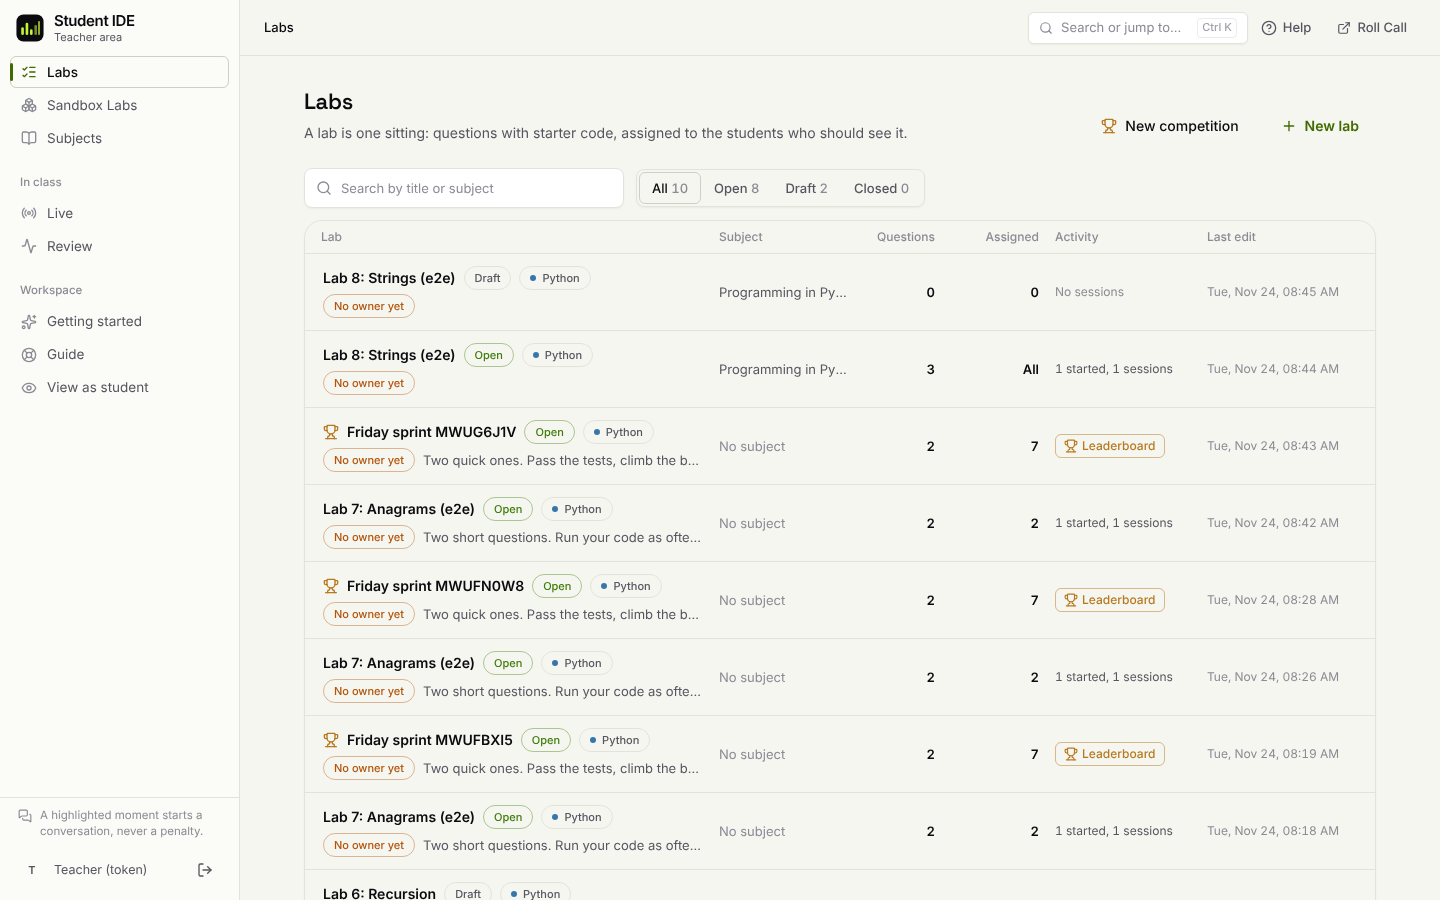
\includegraphics[width=\linewidth]{redesign/acid-night/light-13-teach-labs}
    \caption{A teacher's labs, with the sidebar navigation.}
  \end{subfigure}\\[1ex]
  \begin{subfigure}{0.49\textwidth}
    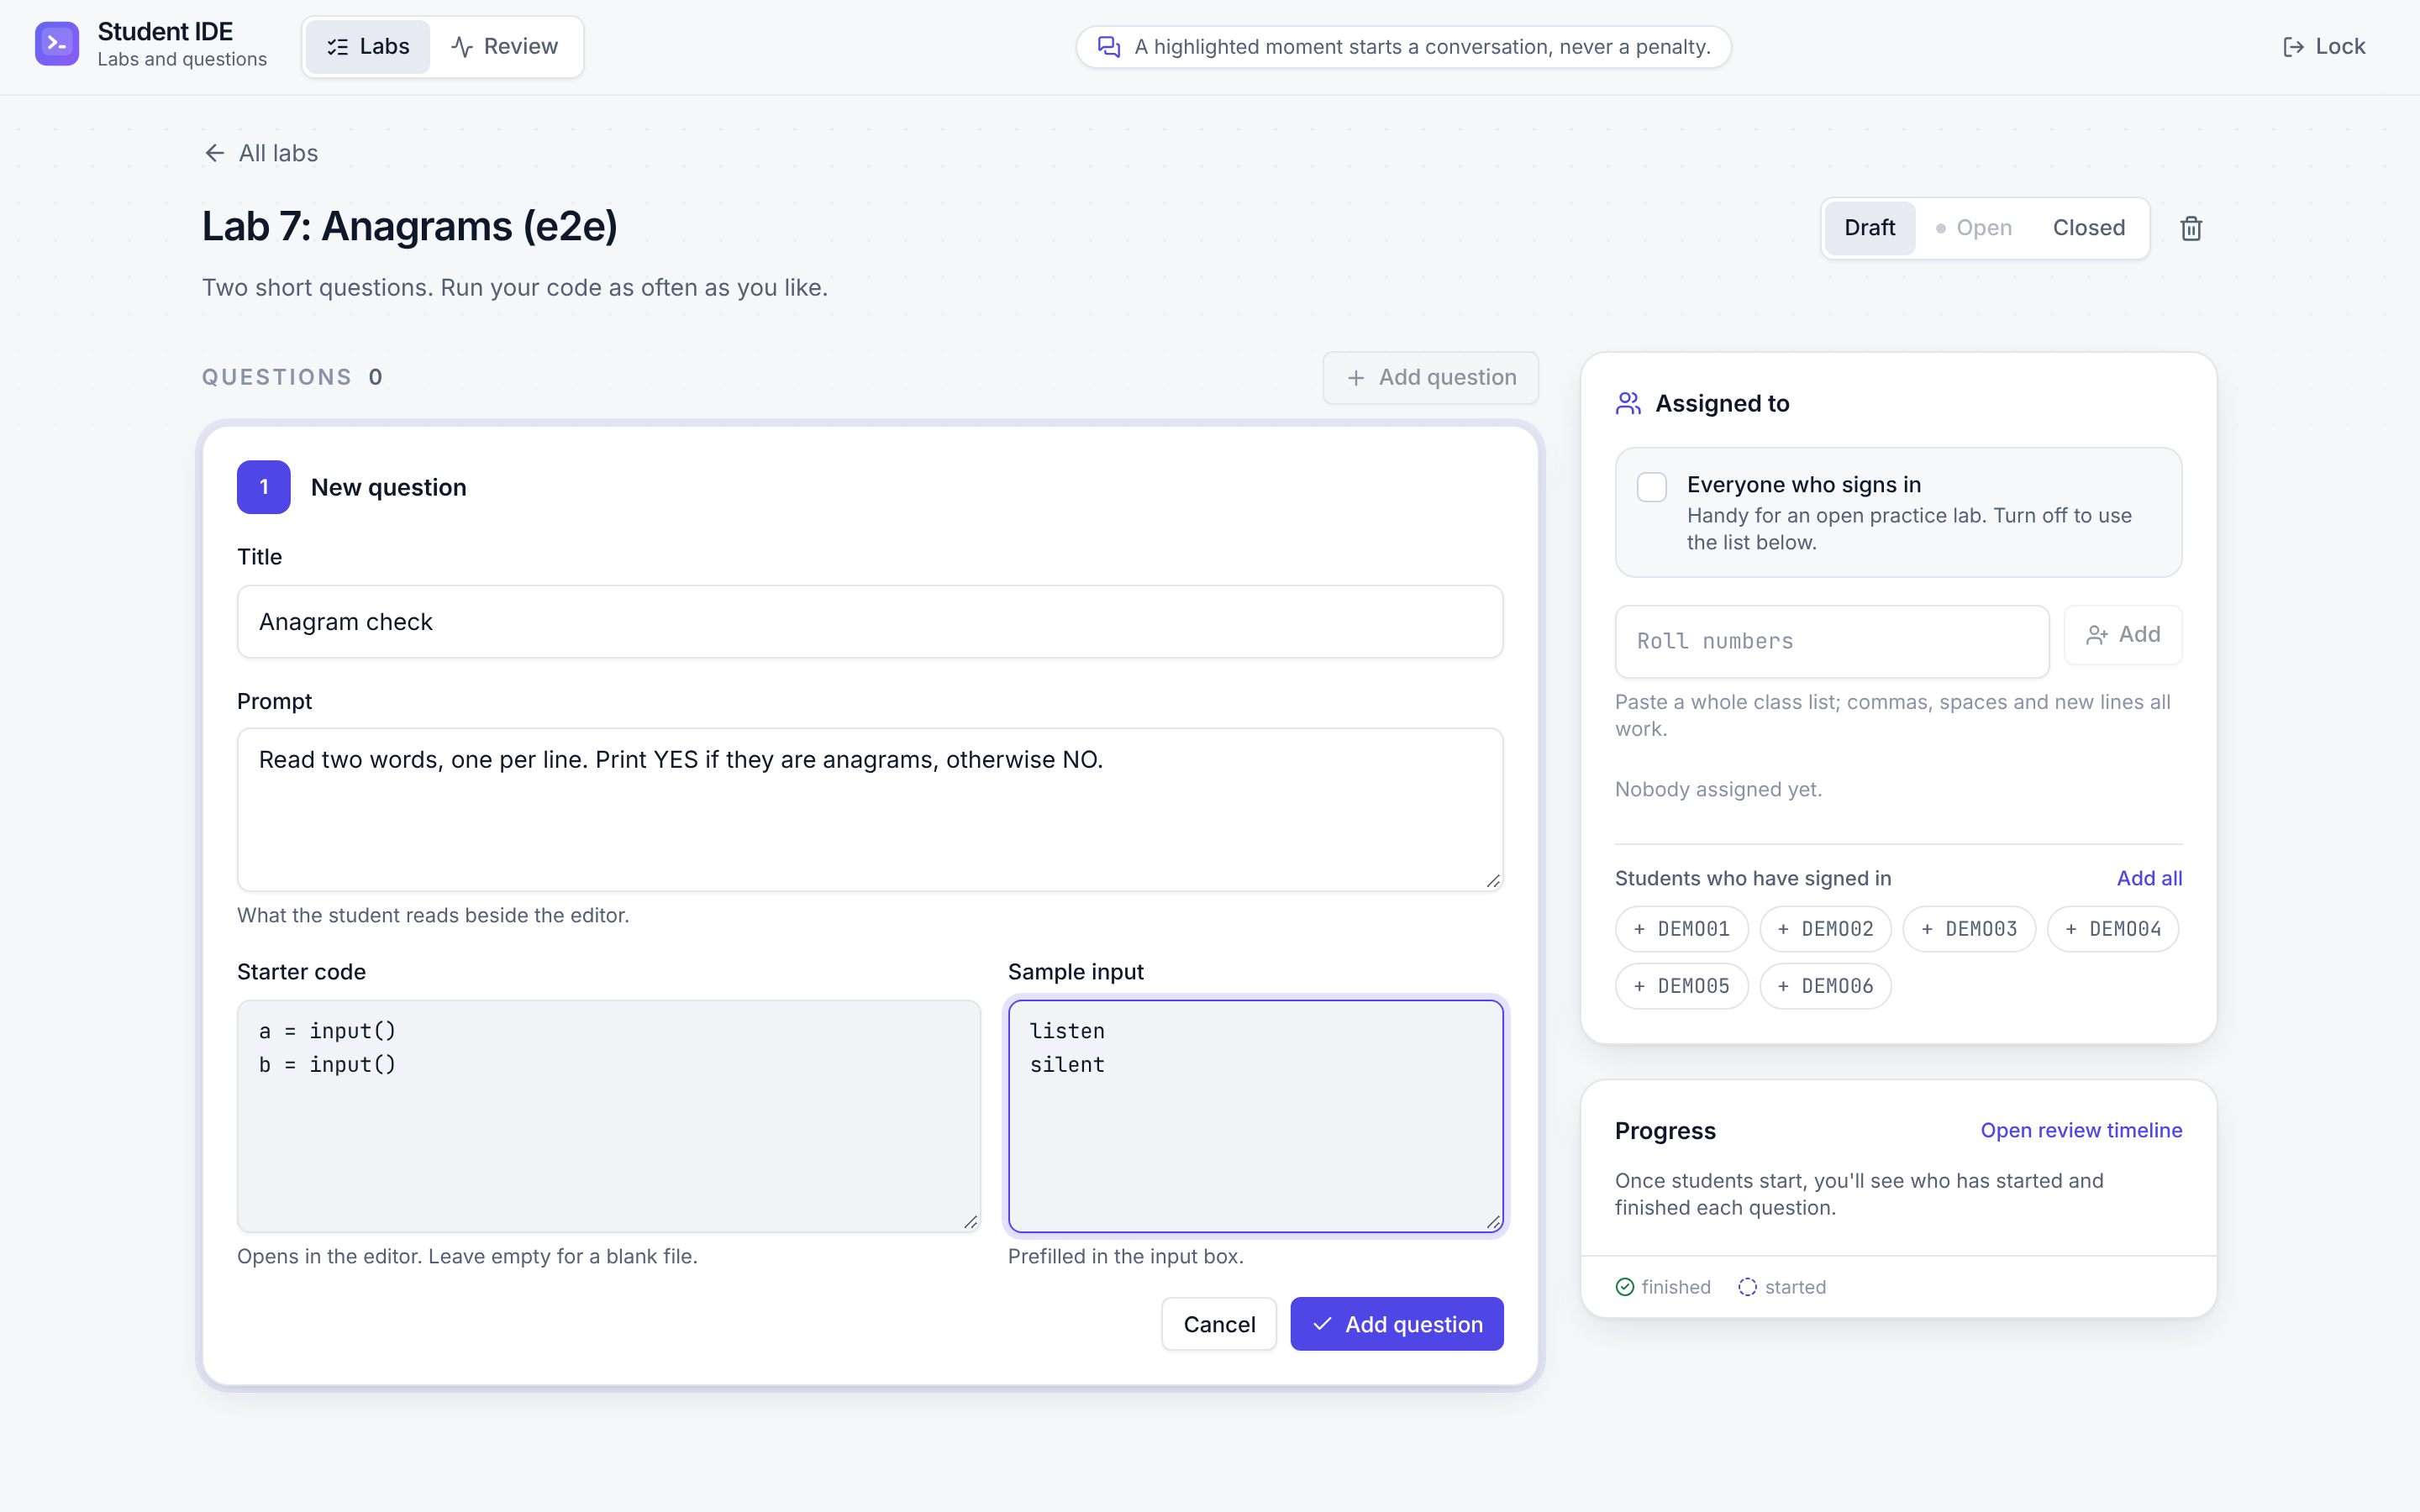
\includegraphics[width=\linewidth]{teach/teach-light-03-question-form}
    \caption{Adding a question.}
  \end{subfigure}\hfill
  \begin{subfigure}{0.49\textwidth}
    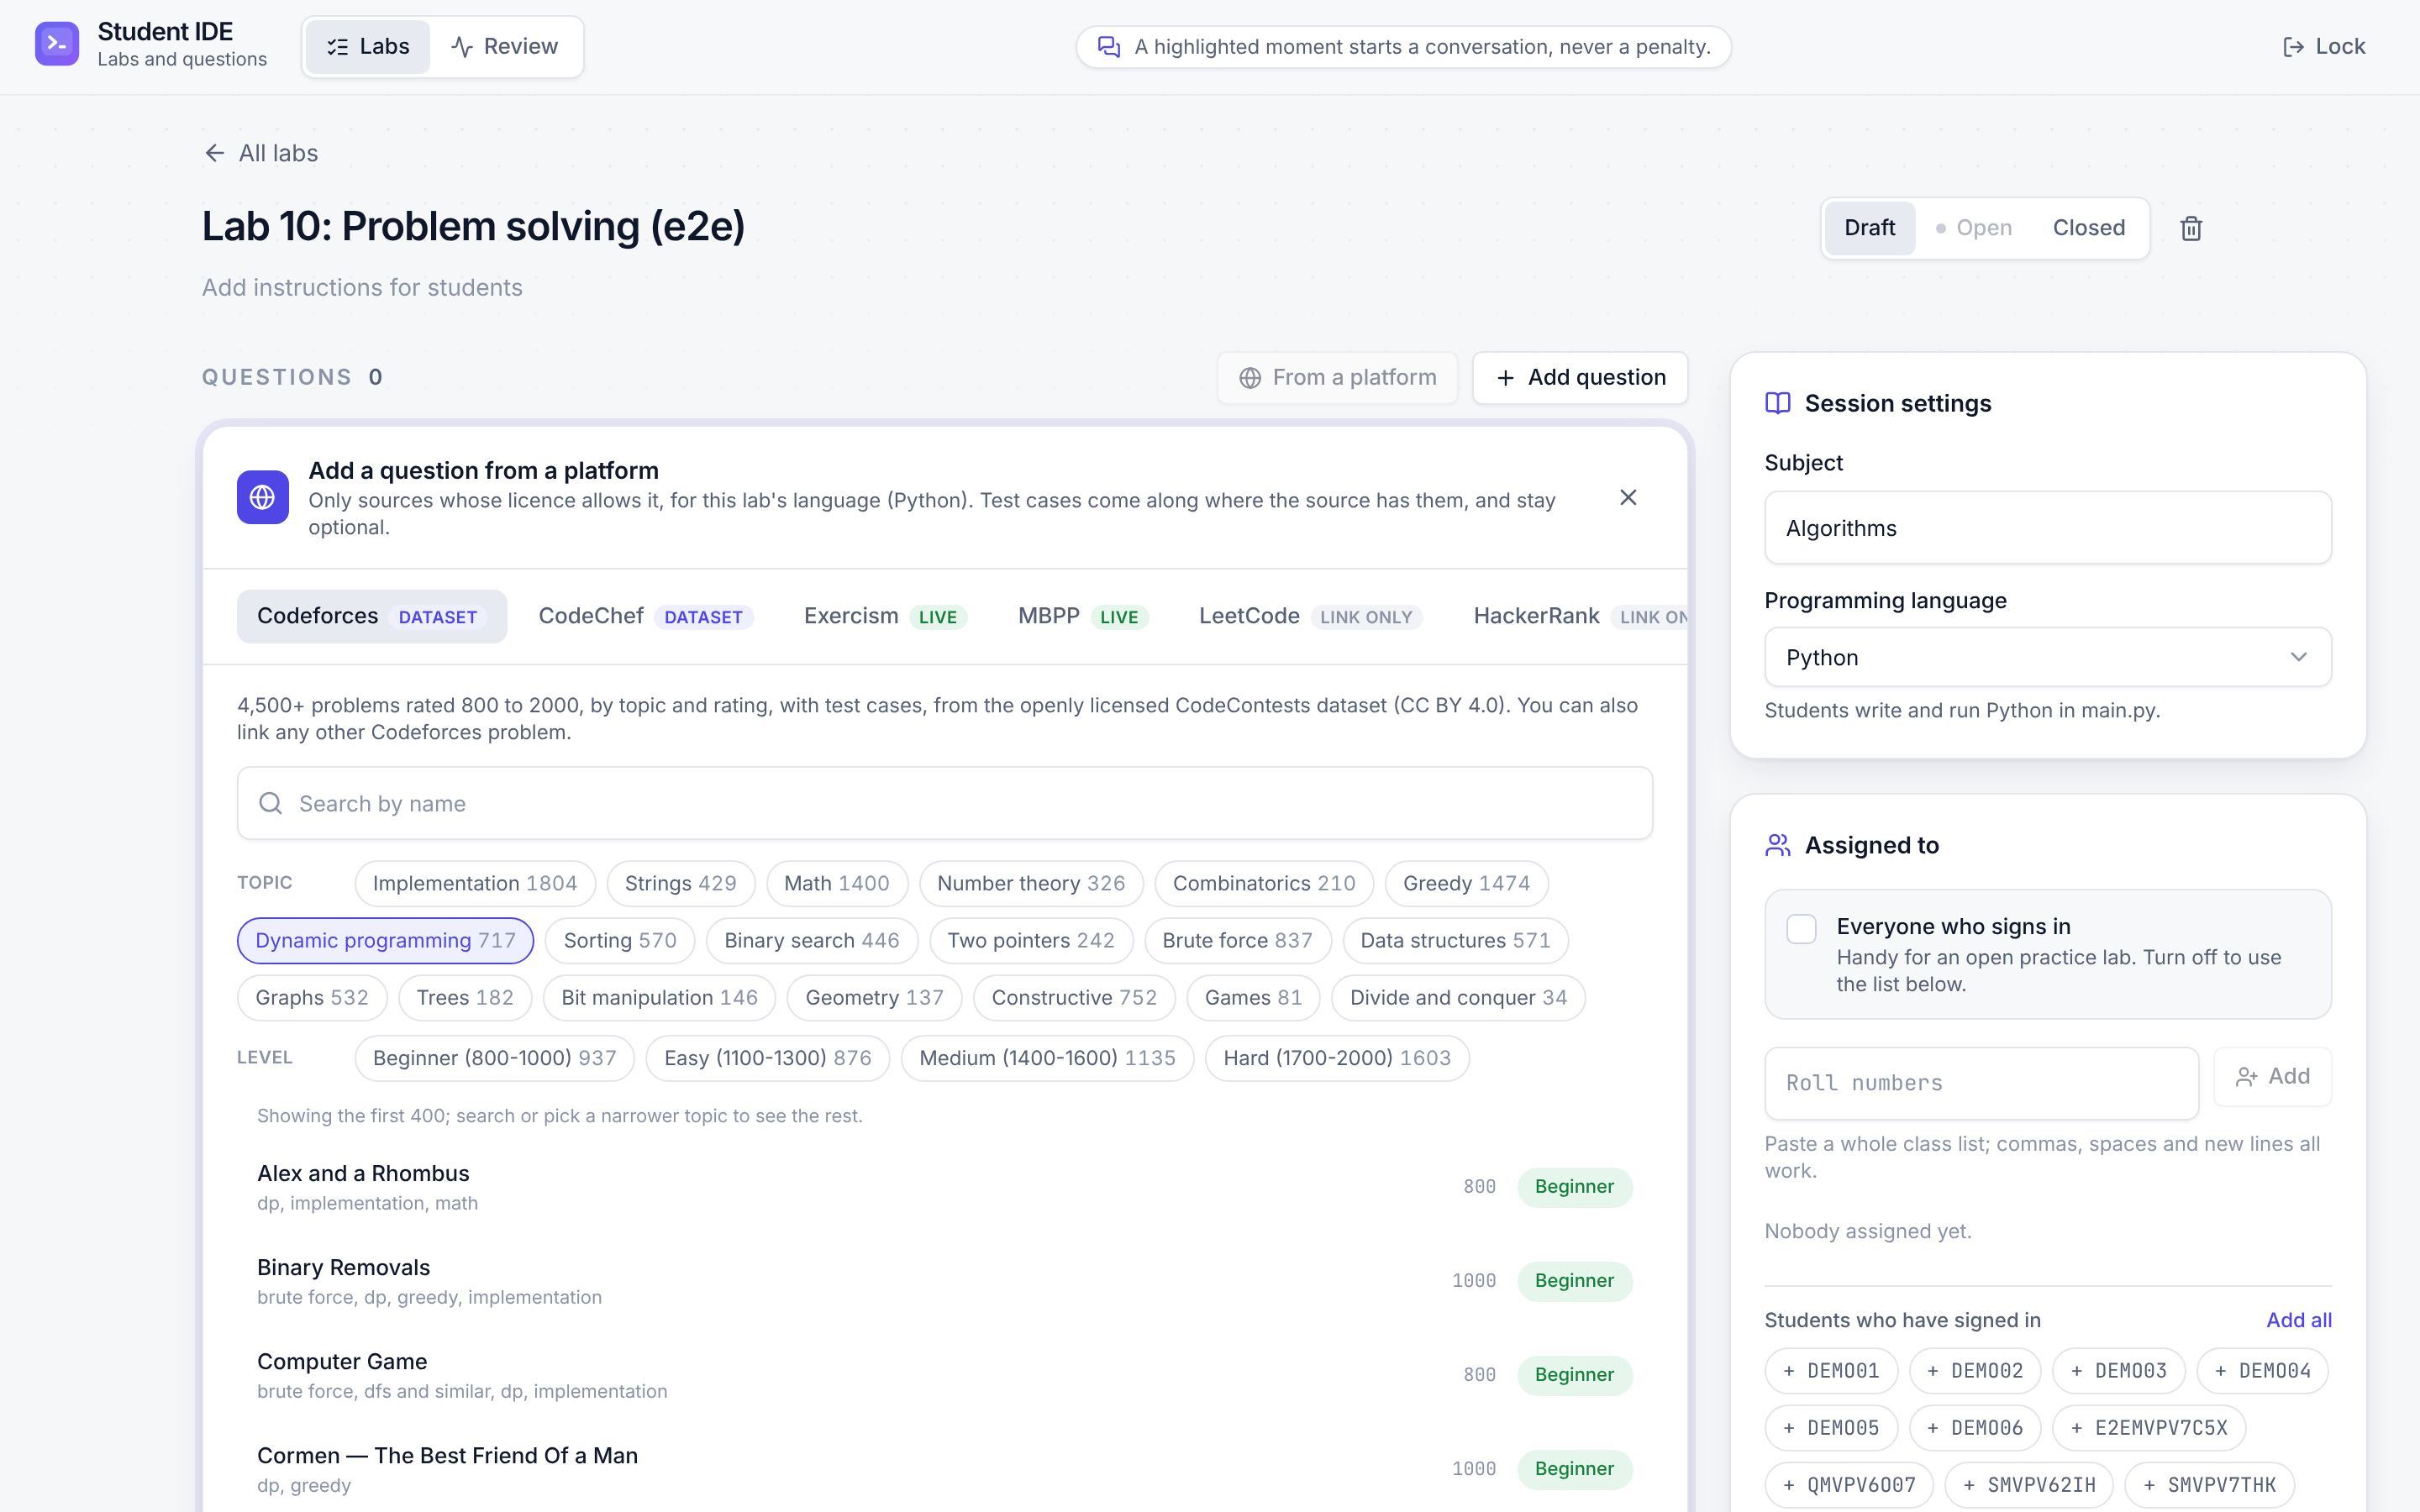
\includegraphics[width=\linewidth]{sources/sources-light-01-codeforces-topics}
    \caption{Codeforces problems by topic and rating.}
  \end{subfigure}
  \caption{Labs and questions.}
  \label{fig:app-teach}
\end{figure}

\section{Class competitions}
A competition is a lab run as a timed, class-wide challenge with a lobby, a
live leaderboard and test-graded submissions (\cref{fig:app-compete}). It is the
one place correctness is scored: $100\times$ the share of tests passed, plus up
to 50 points for a full solve scaled by the time left; wrong submissions cost
nothing. The board is gentle by design (the top ten and the student's own
place, never who is last; chosen board names only; badges so that more
students stand out) and reads nothing from the detector, so a moment flagged
for conversation can never cost a place or become public. When the clock ends,
each student's last code is rebuilt from the edit log and graded as a hand-in,
so working code that was never submitted still counts. A competition can allow
any language per question. Competition sessions are kept out of the lab
baseline (\cref{sec:non-study}).

For teachers, a \emph{similar submissions worth a look} page compares final
submissions with winnowed fingerprints \cite{schleimer2003winnowing} and
greedy string tiling \cite{wise1993gst,prechelt2002jplag} after masking starter
code and stretches most of the class wrote alike. It shows the common
stretches and how each program got into the editor (typed and pasted
characters), never says ``copied'', and never touches a score. On six contest
problems solved independently three times each, no independent pair reached
0.4 while every disguised copy scored at least 0.67
(\cref{tab:similarity-separation}); these independent solutions were written
by one author in deliberately different styles, so real classmates will
overlap more.

% Generated by backend/scripts/eval_similarity.py. Do not edit by hand.
\begin{table}[ht]
  \centering\small
  \caption{Similarity check on six contest problems, each solved independently three times in C/C++ and
    three times in Python. Each solution was also copied with increasing disguise. Columns on the right:
    share of pairs at or above each similarity (the page lists pairs from 0.3 and highlights from 0.5).}
  \label{tab:similarity-separation}
  \begin{tabular}{@{}lrcccccc@{}}
    \toprule
    Pairs & $n$ & Median & Range & $\ge 0.4$ & $\ge 0.5$ & $\ge 0.6$ & $\ge 0.7$ \\
    \midrule
    Independent solutions & 36 & 0.00 & 0.00--0.36 & 0\% & 0\% & 0\% & 0\% \\
    Copy: renamed + reformatted & 36 & 1.00 & 0.83--1.00 & 100\% & 100\% & 100\% & 100\% \\
    Copy: + rewritten constructs & 36 & 0.98 & 0.77--1.00 & 100\% & 100\% & 100\% & 100\% \\
    Copy: + dead code every 3rd line & 36 & 0.93 & 0.67--1.00 & 100\% & 100\% & 100\% & 97\% \\
    \bottomrule
  \end{tabular}
\end{table}


\begin{figure}[ht]
  \centering
  \begin{subfigure}{0.49\textwidth}
    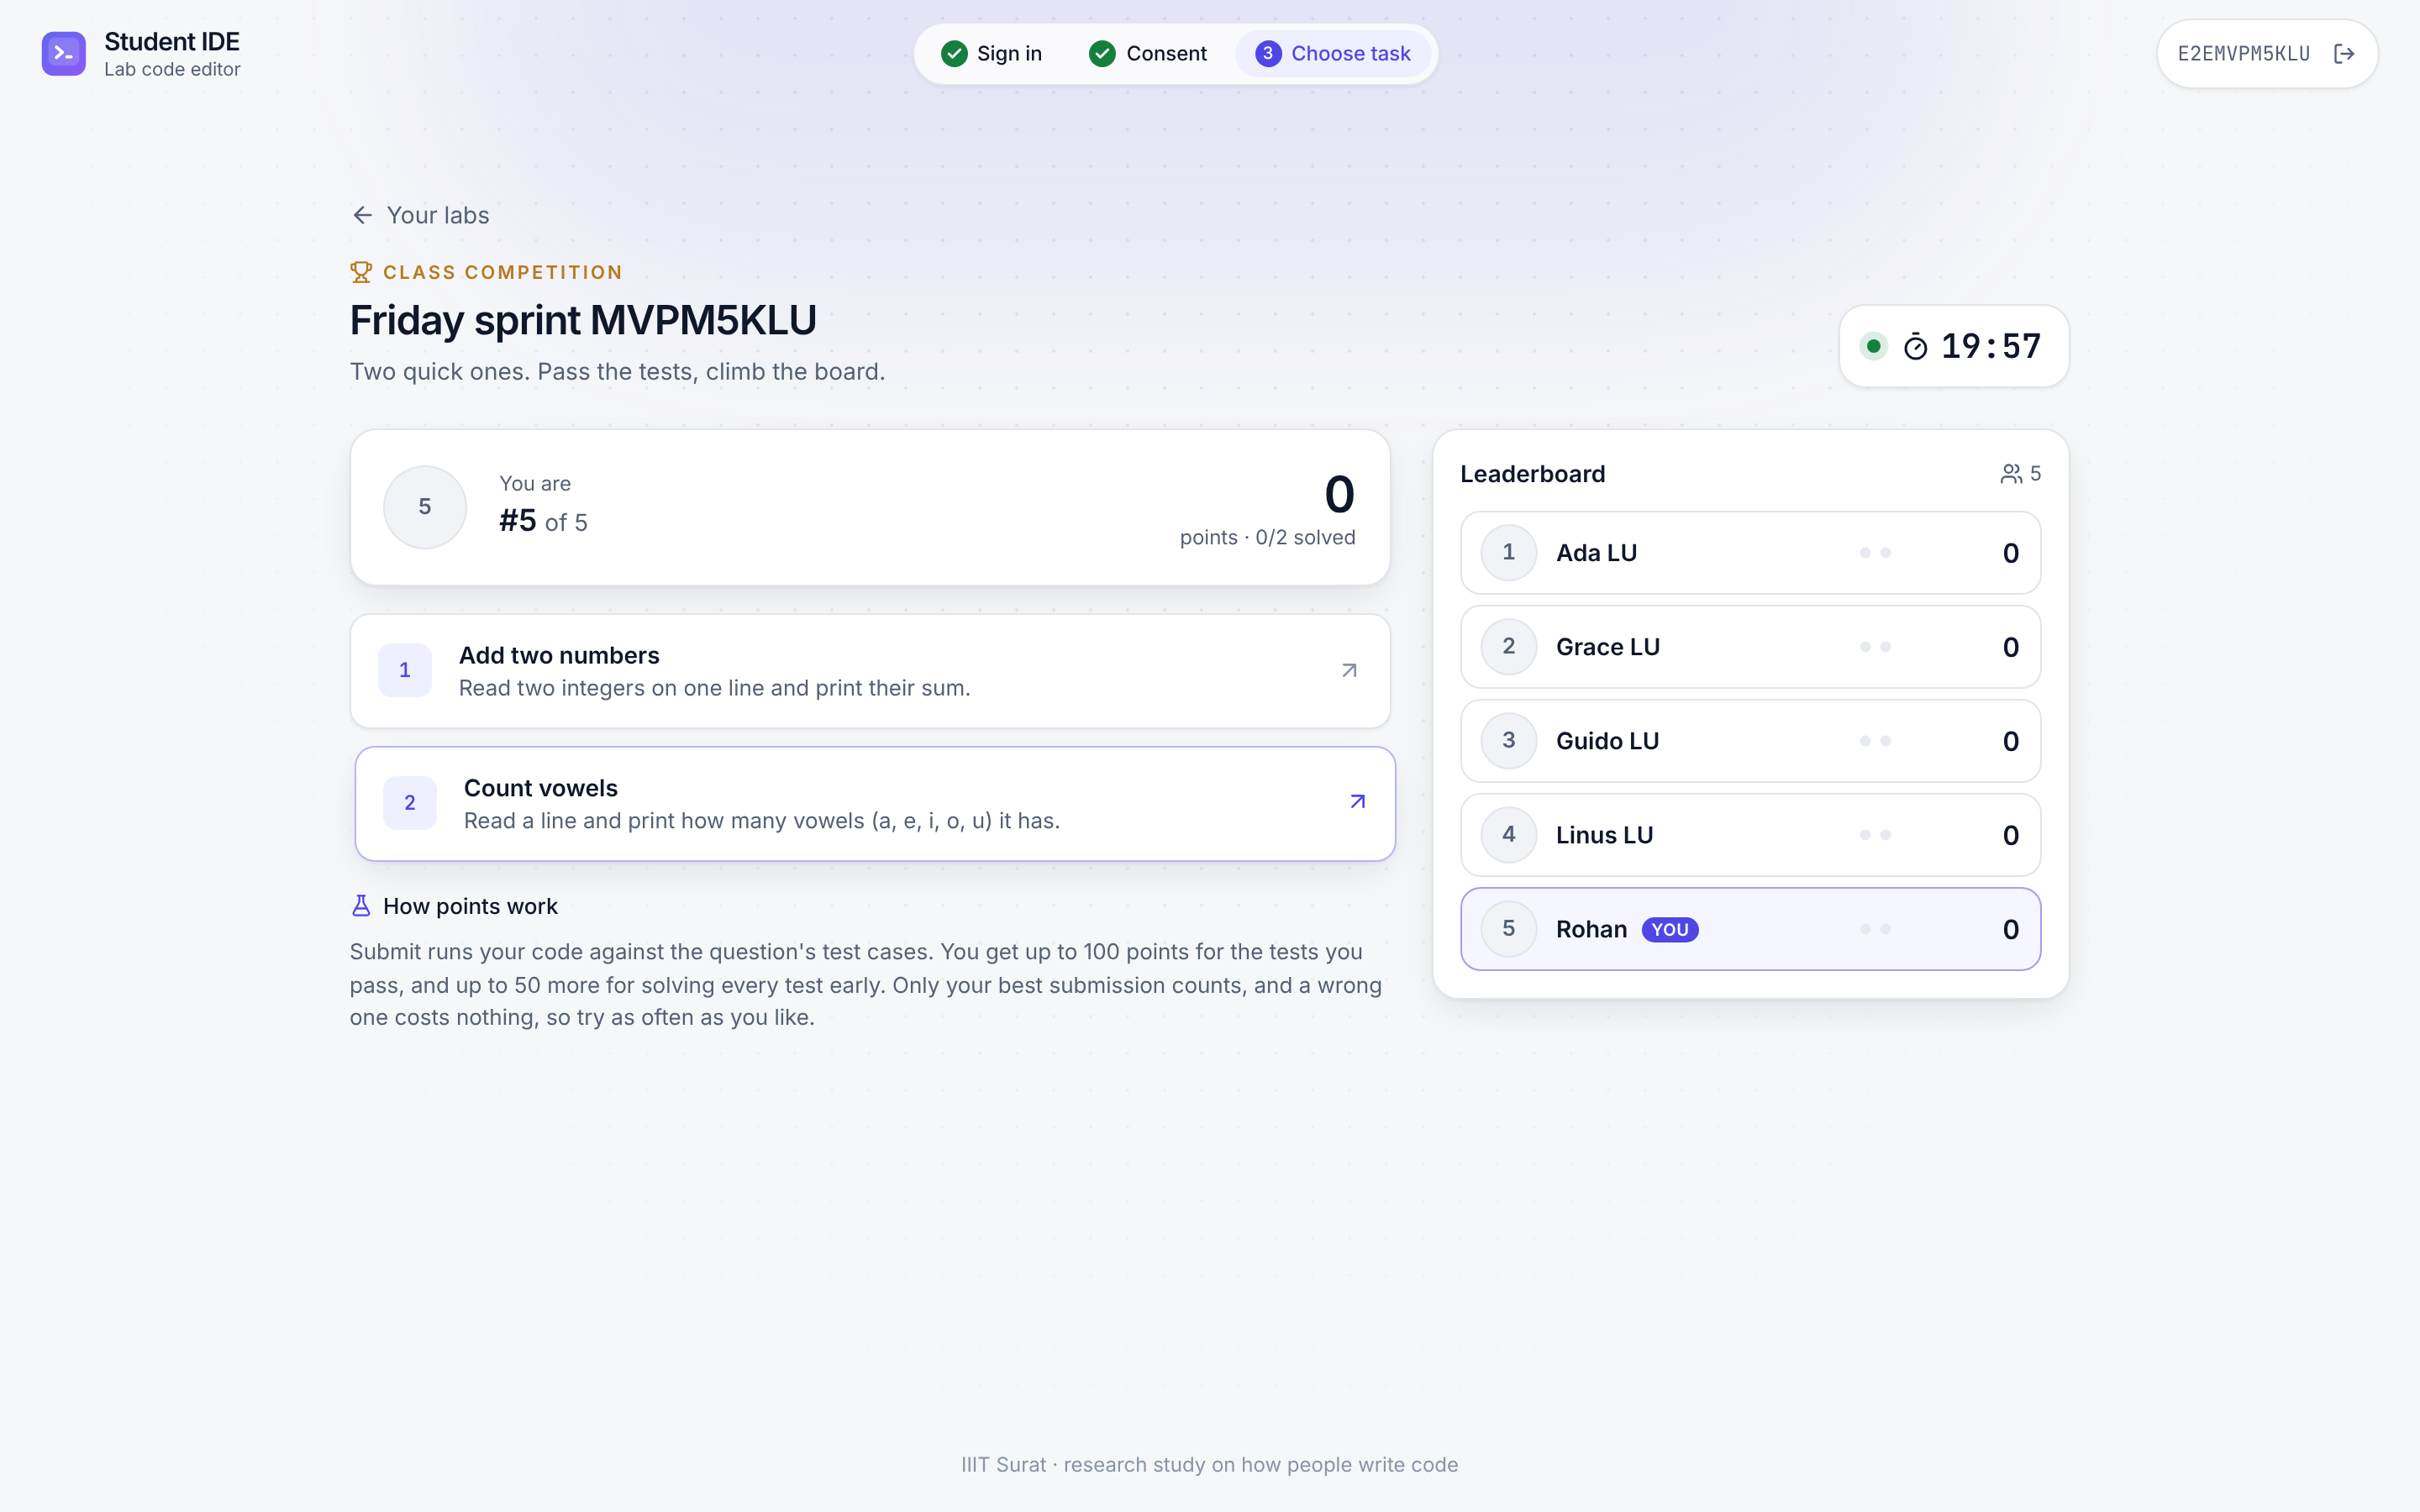
\includegraphics[width=\linewidth]{compete/compete-light-05-arena-live}
    \caption{A student's view during a competition.}
  \end{subfigure}\hfill
  \begin{subfigure}{0.49\textwidth}
    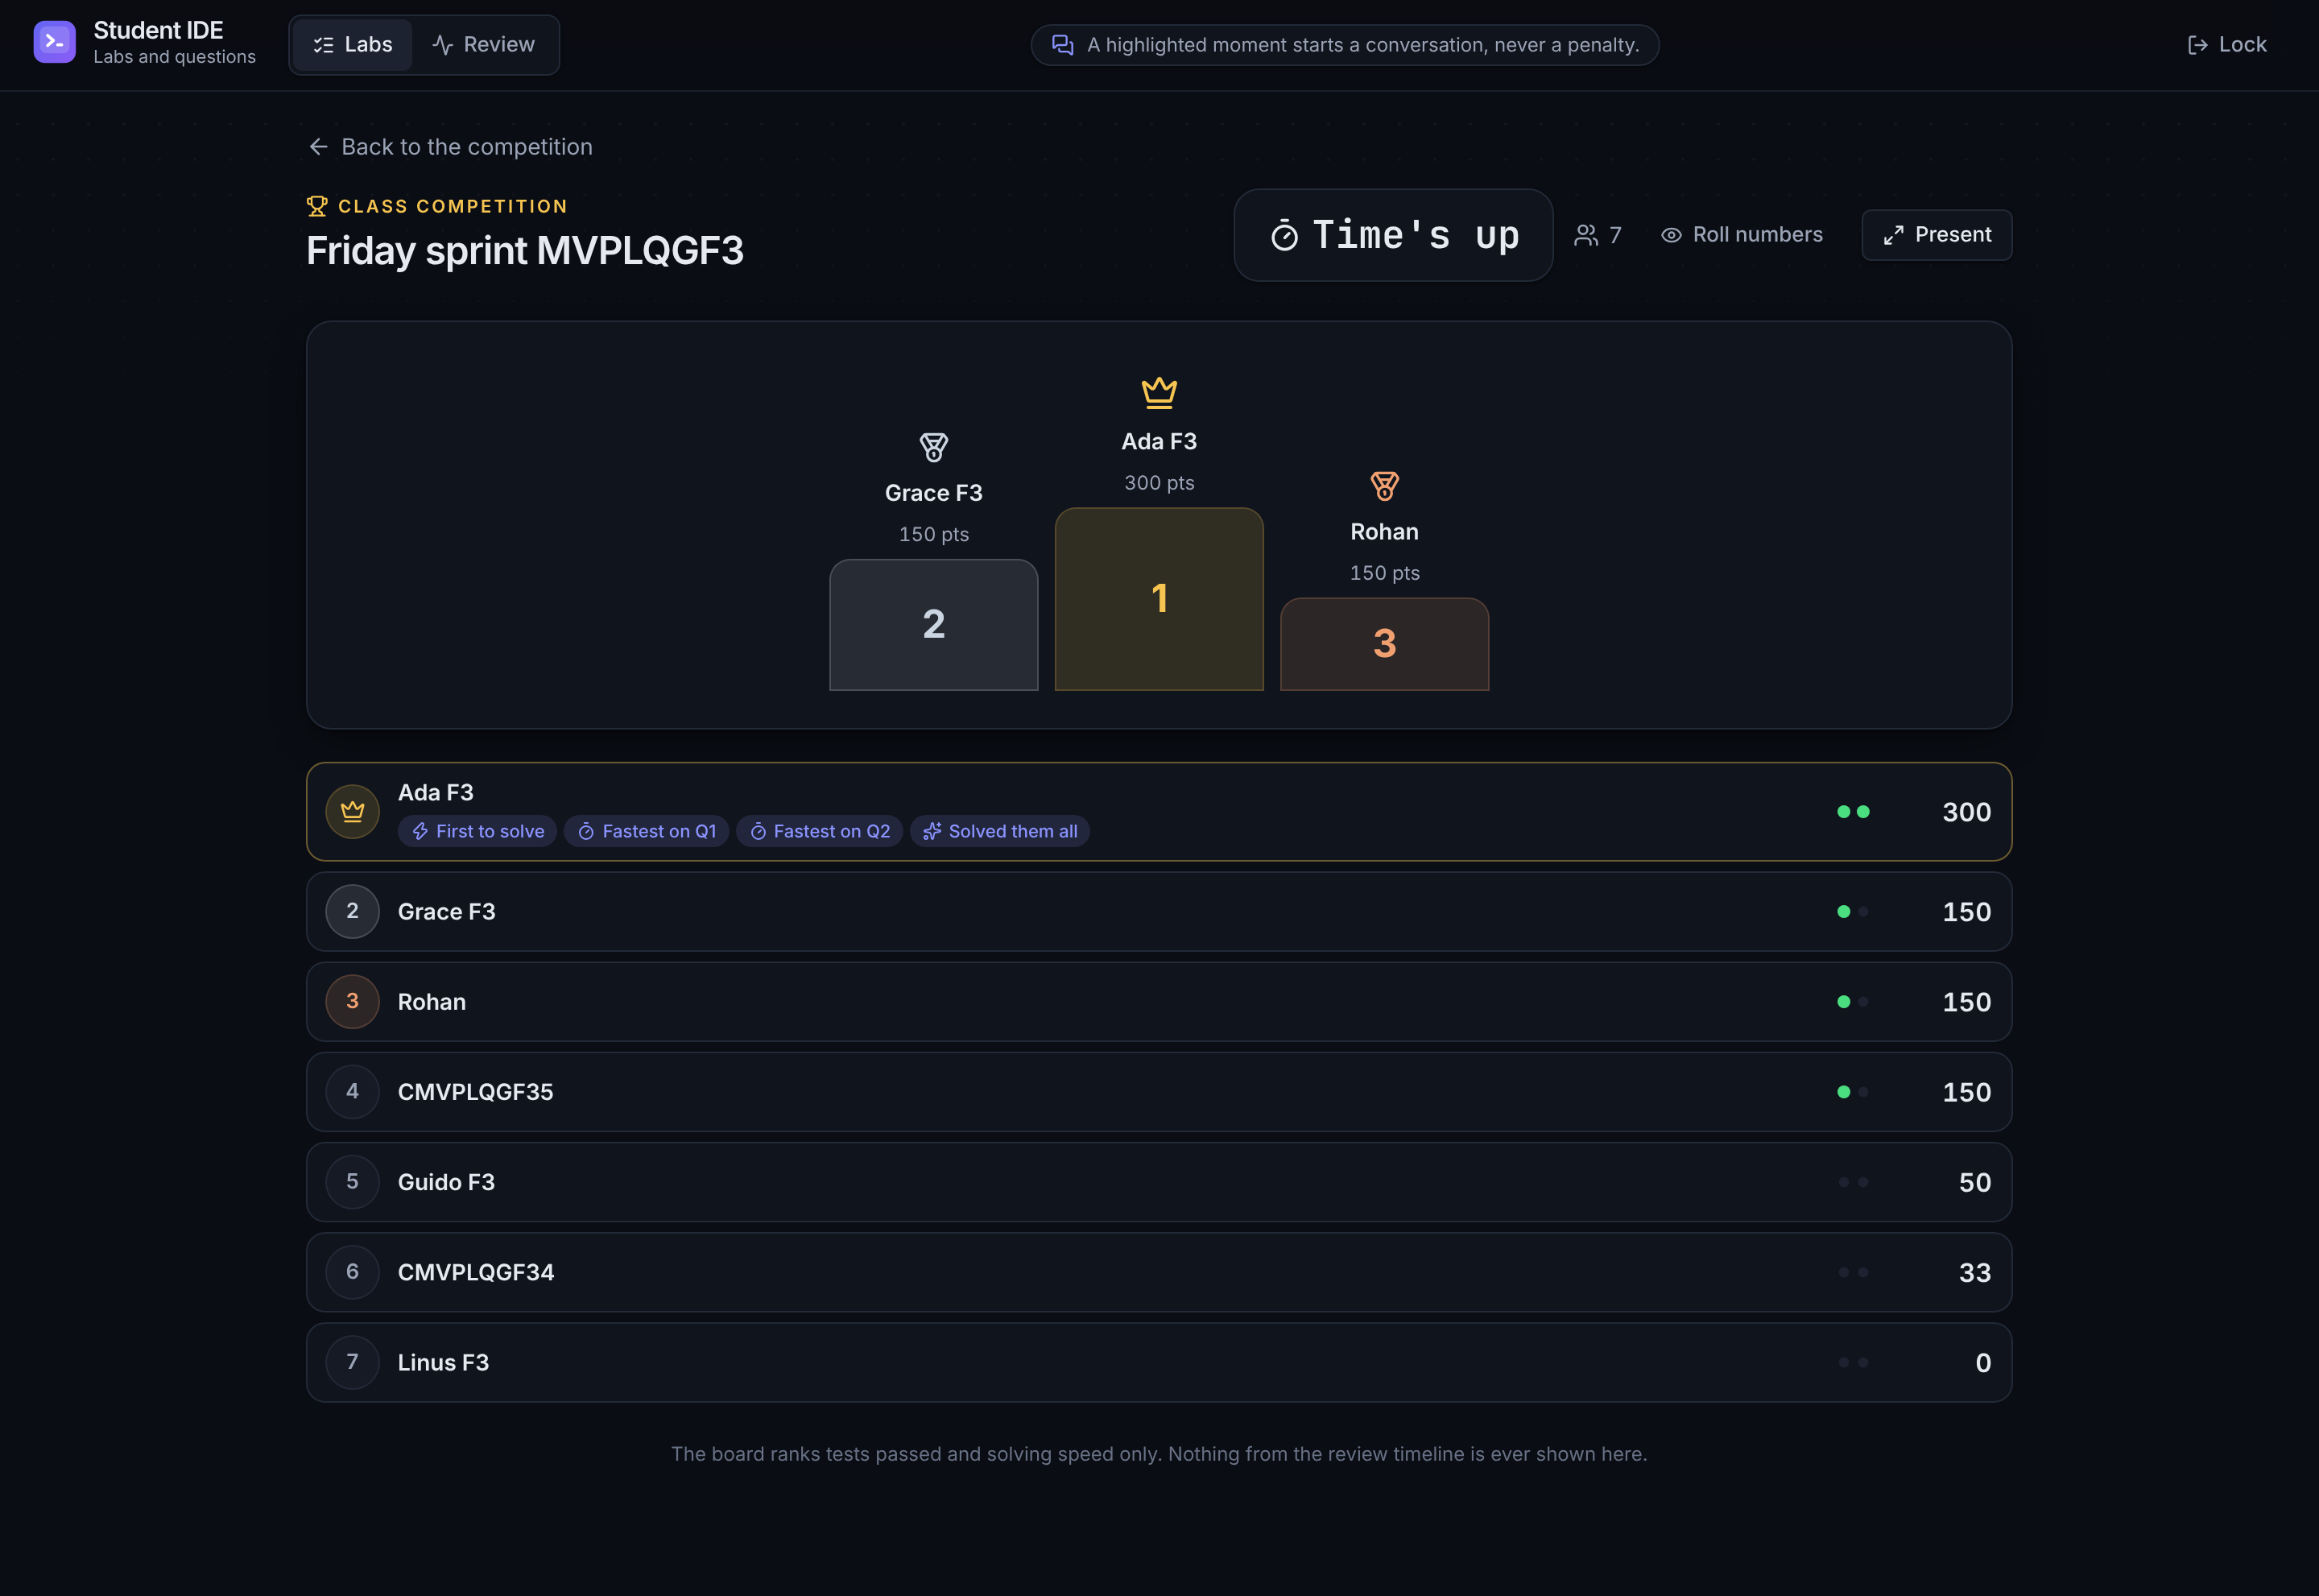
\includegraphics[width=\linewidth]{compete/compete-dark-09-podium}
    \caption{The projector board at the end.}
  \end{subfigure}\\[1ex]
  \begin{subfigure}{\textwidth}
    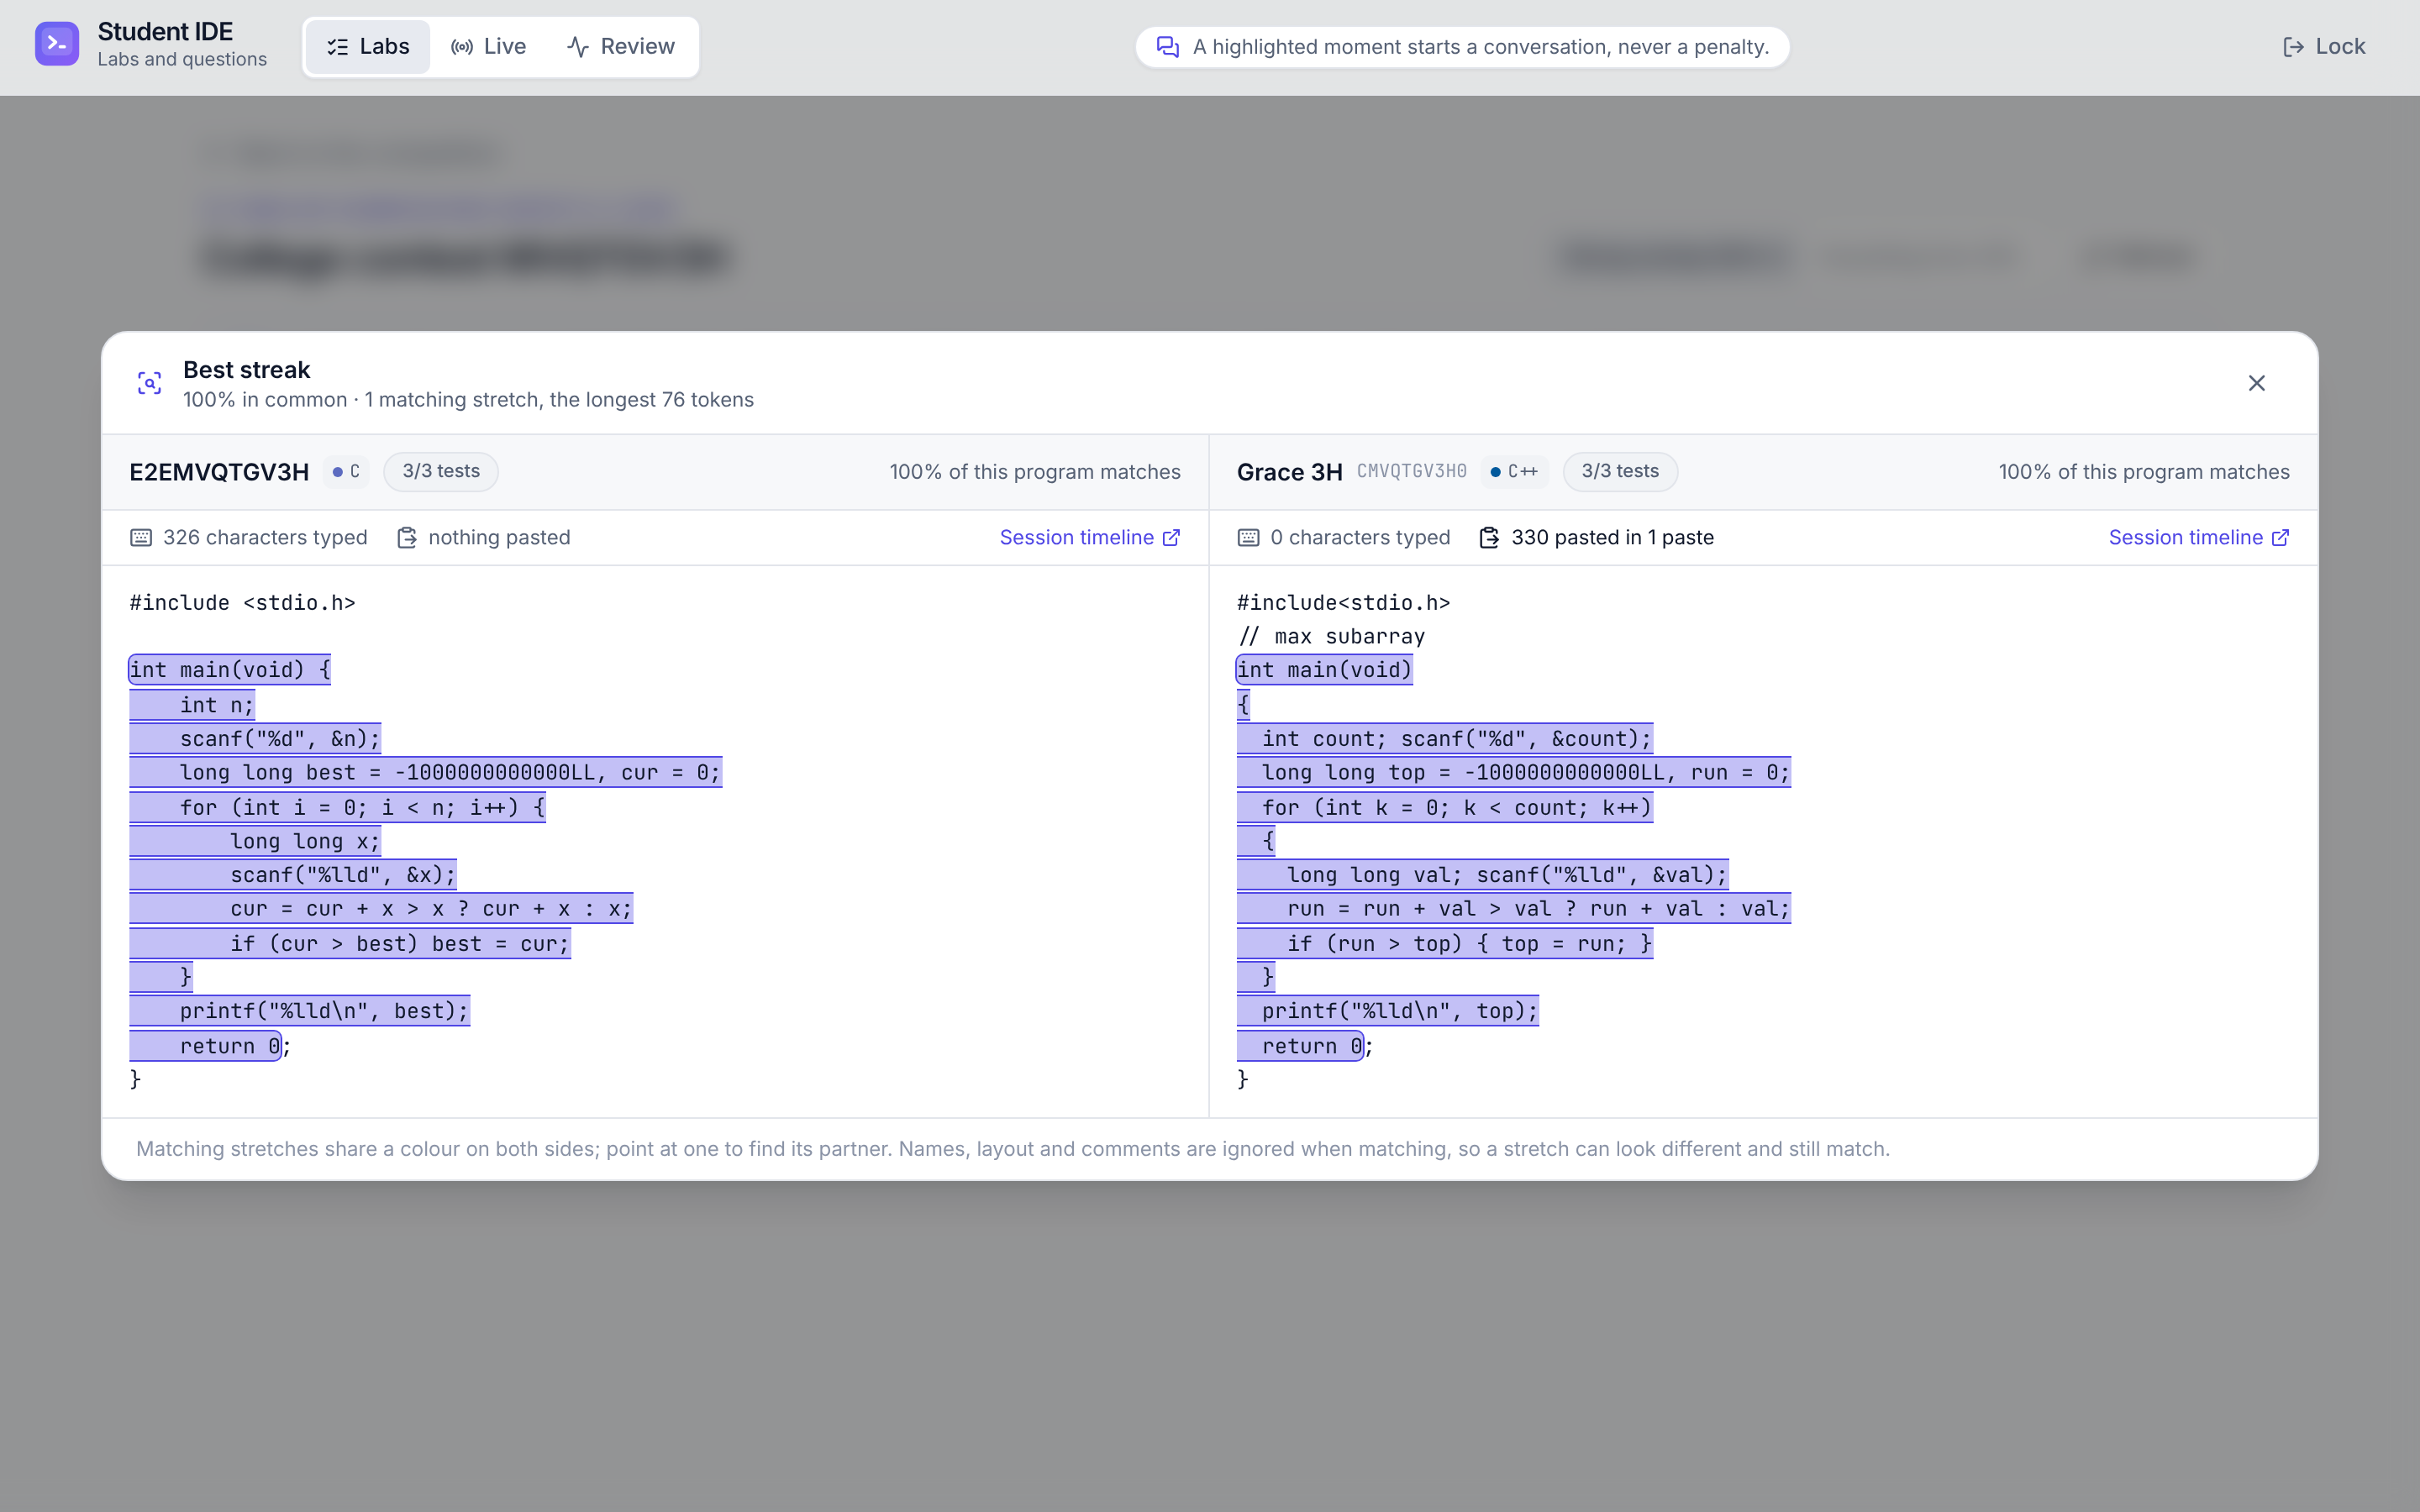
\includegraphics[width=\linewidth]{anylang/anylang-light-08-similar-pair}
    \caption{A similar pair side by side, with typed and pasted characters.}
  \end{subfigure}
  \caption{Class competitions and the similar-submissions page.}
  \label{fig:app-compete}
\end{figure}

\section{Live classroom view}
During a lab, a teacher mostly wants to know who is stuck. A \emph{Live} view
uses the events the editor already uploads every two seconds to show one card
per student: whether they are typing, working, quiet or away, the question
they are on, recent edits, runs and the last error, test checks, and any
moments found so far (\cref{fig:app-live}). It shows no code. A teacher can open
a read-only copy of one student's editor, rebuilt from the edit events. Viewing
is never silent: that student's editor names the teacher while they watch,
every student sees a notice while the class view is open, each view is logged,
and the consent text says so (\cref{app:consent}). A server setting limits the
feature to the class view or turns it off. No new data is recorded for it.

\begin{figure}[ht]
  \centering
  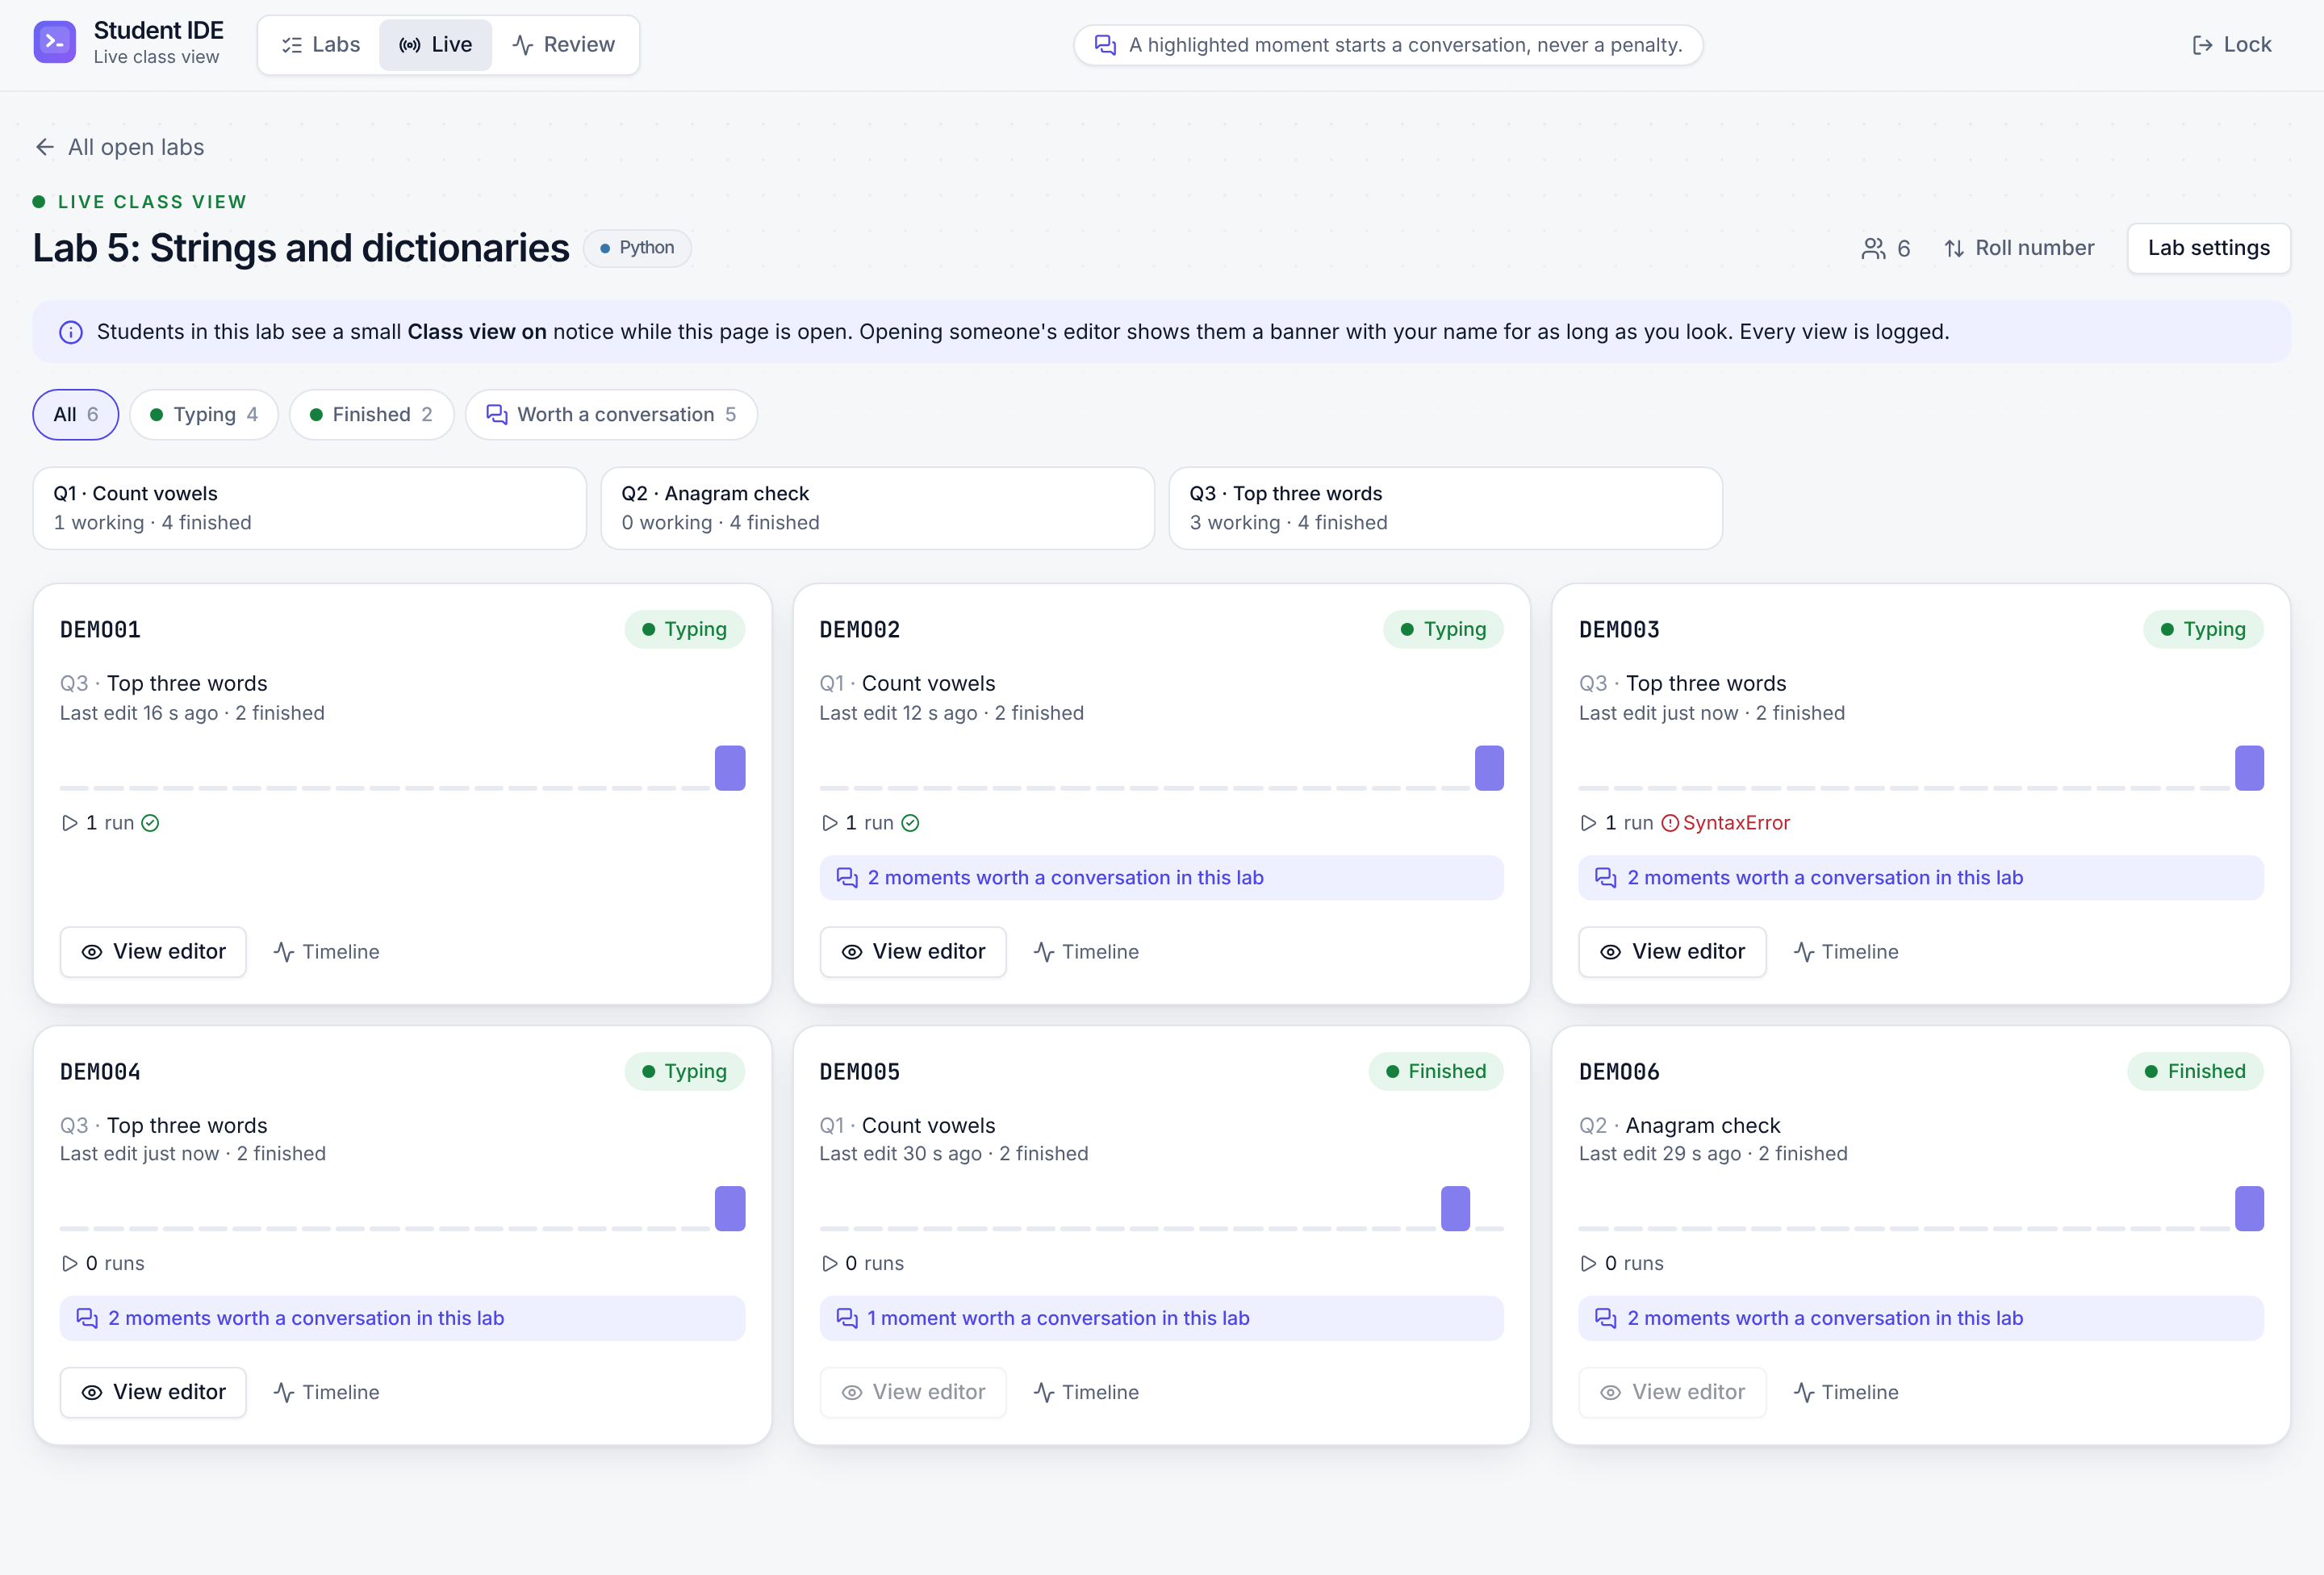
\includegraphics[width=\linewidth]{live/live-light-03-class}
  \caption{Live class view: state, question, recent activity, runs, checks and
  moments per student. No code is shown.}
  \label{fig:app-live}
\end{figure}

\section{Learning lab and staff previews}
An always-open \emph{learning lab} has 82 short lessons in eight tracks (C,
C++ and Python, beginner to advanced), each explaining one idea beside code the
student can change and run and ending with an exercise checked by the same
tests as lab questions (\cref{fig:app-learn}). Lessons are Markdown files whose
model answers are run by an automated test. Practice opens in the same editor
as a lab, but it is unsupervised and could be typed by anyone, so it is marked
as such and kept out of baselines, the detector, review, the live view and the
evaluation. \emph{View as student} lets staff try a lab, including a draft,
under their own account; those sessions are marked as previews by the server
and excluded in the same way.

\begin{figure}[ht]
  \centering
  \includegraphics[width=\linewidth]{learn/learn-light-04-exercise-checked}
  \caption{A learning-lab lesson: text and examples beside the editor; the
  exercise passes its check.}
  \label{fig:app-learn}
\end{figure}

\section{Attendance through Roll Call}
Lab classes need an attendance register, which the department keeps in a
separate application, Roll Call. Rather than have teachers take a roll call
during a recorded lab, Scribelab marks it. A lab attaches one or more Roll Call
class groups; when the teacher closes the lab, each student on those rosters is
marked present or absent for the day (\cref{fig:app-attendance}). A student
counts as present only with at least ten active minutes (distinct minutes with
an edit, run or check) and forty typed characters; pasted text and resets do
not count. The rule reads edit, run and check records only, so it works after
raw keys are deleted, and it is independent of the detector: a highlighted
moment never changes attendance. The teacher sees the reason for each mark and
can override it before sending. Students can see their own marks, and nothing
else, in Roll Call.

\begin{figure}[ht]
  \centering
  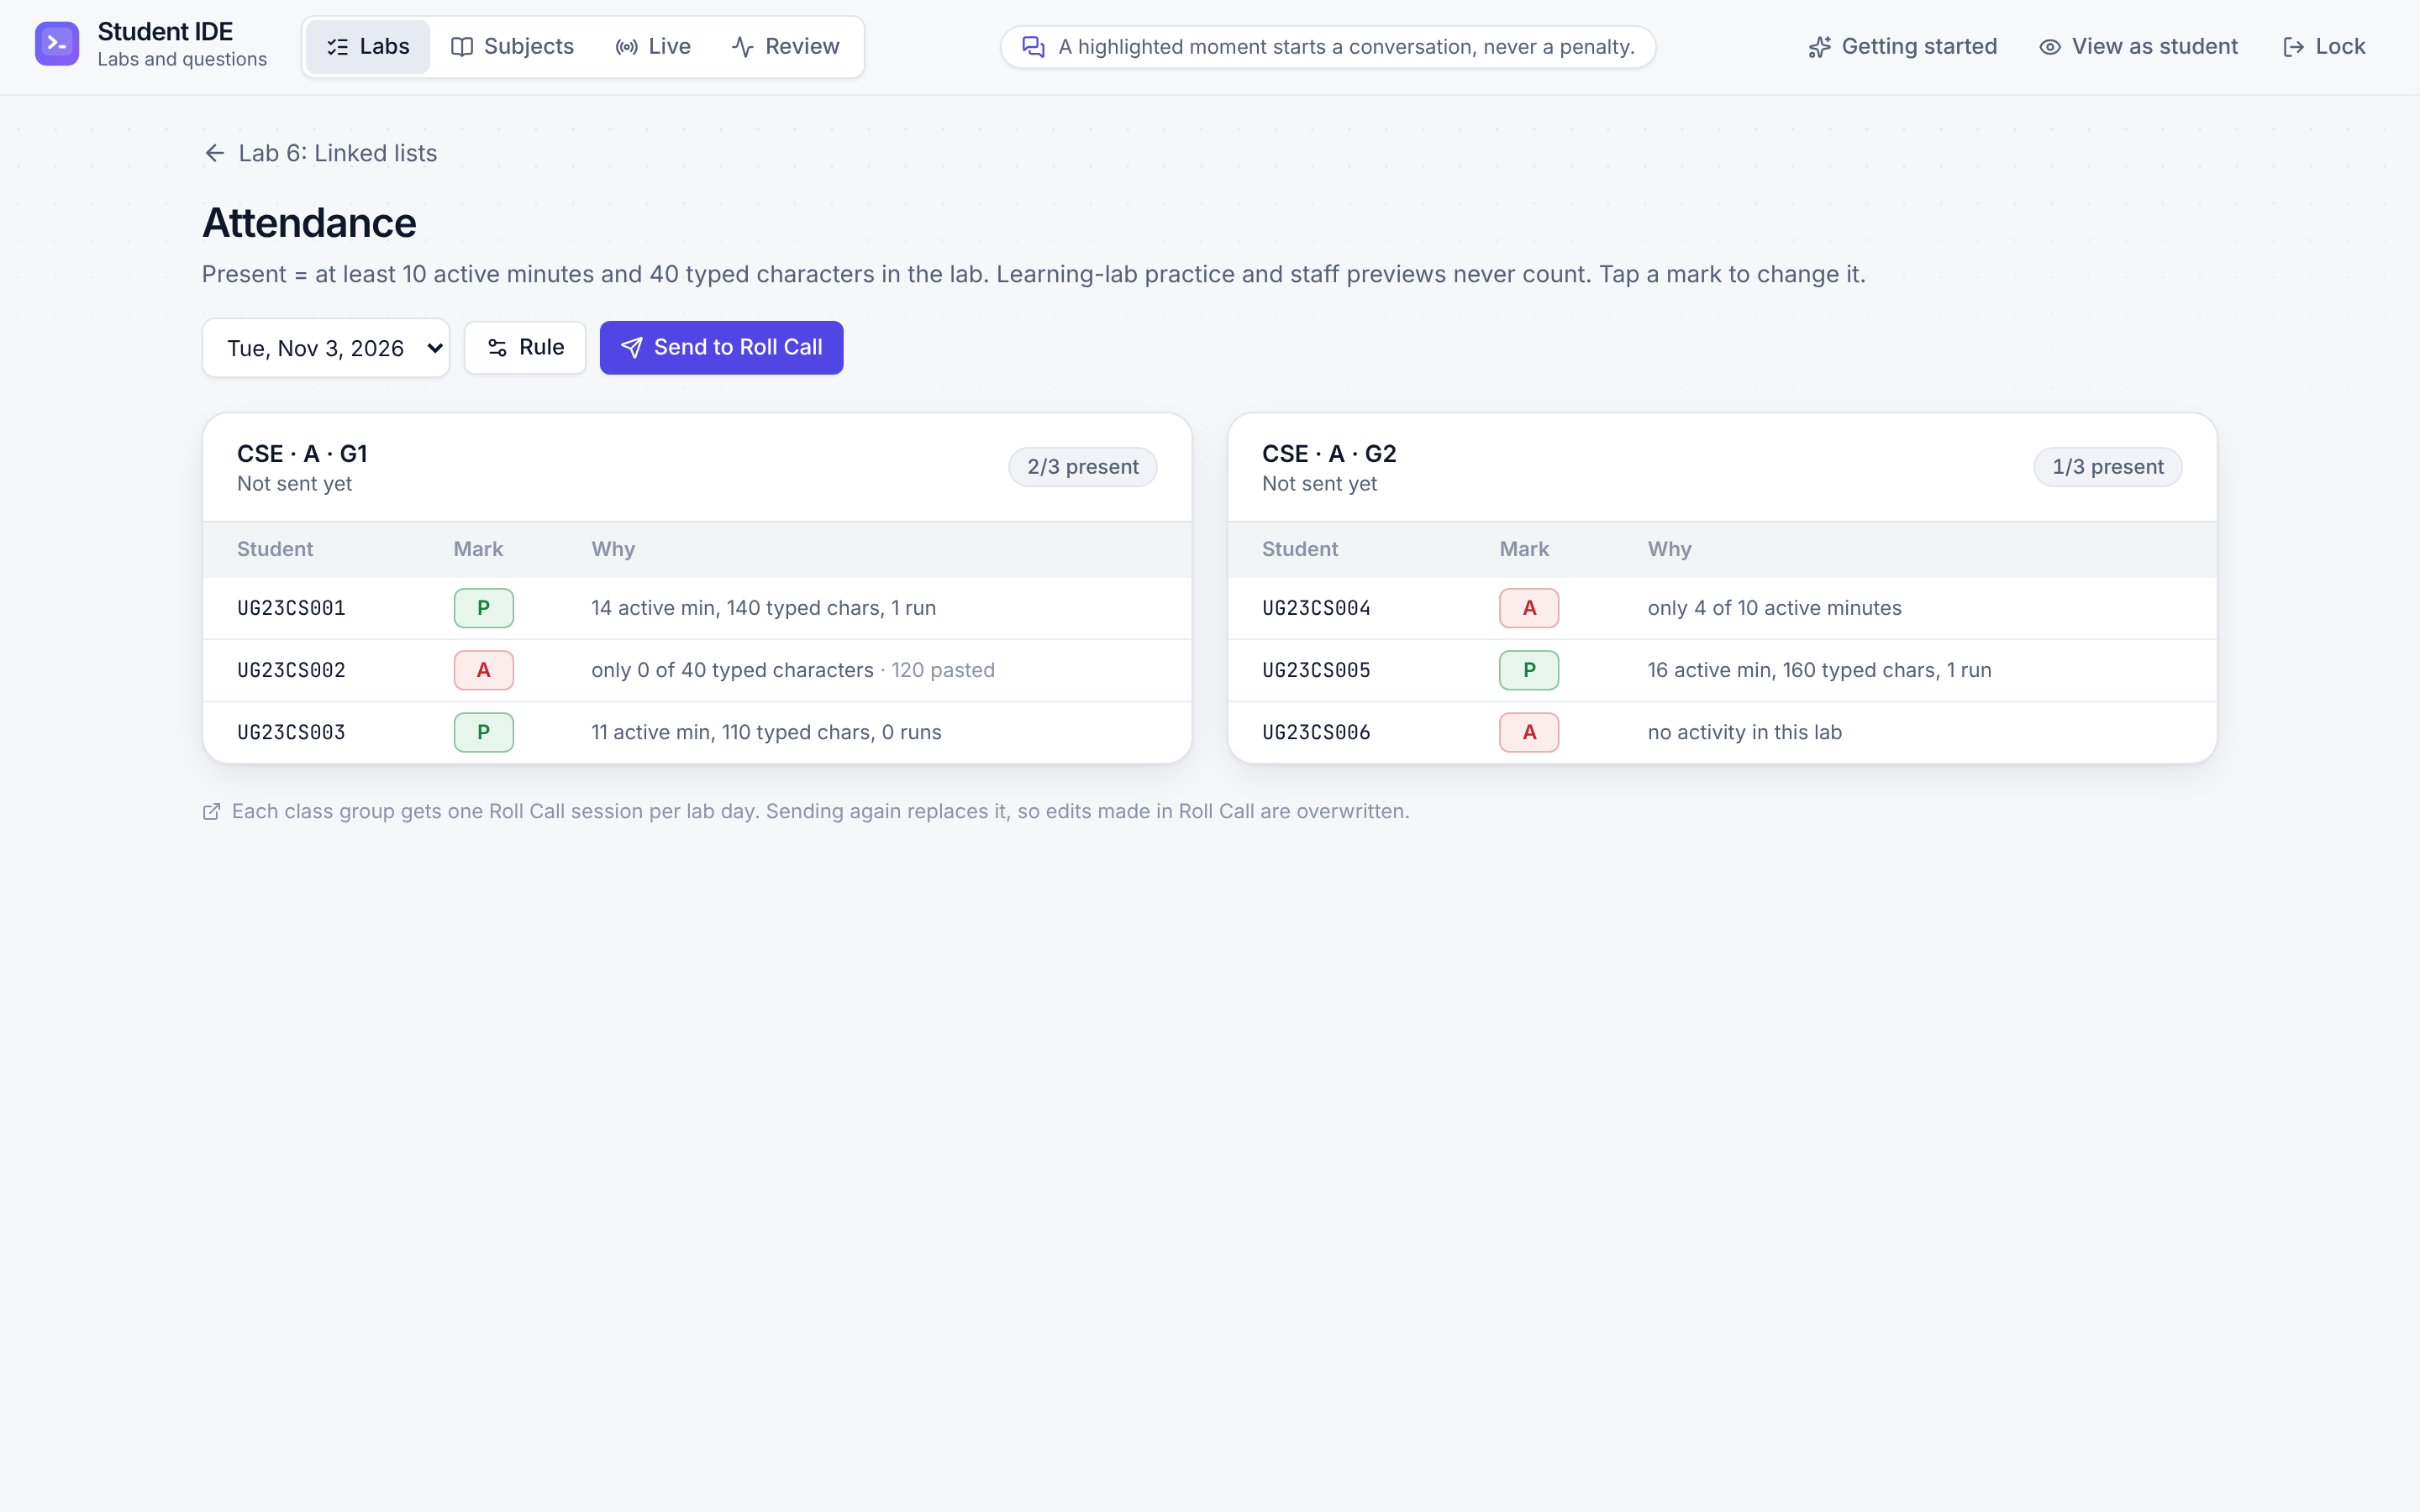
\includegraphics[width=\linewidth]{attendance/attendance-light-04-preview}
  \caption{A lab's attendance page: one card per class group, each mark with
  its reason.}
  \label{fig:app-attendance}
\end{figure}

\section{Interface and desktop app}
The interface was redesigned twice without changing what is recorded: once
after the logger worked, and again in November 2026 into one product with a
sectioned teacher sidebar, a \emph{Ctrl+K} jump list, one page recipe, and
in-app guides for students and teachers. Its look is deliberately quiet and
border-based, with no motion inside the editor. The desktop app (Windows,
macOS, Linux) wraps the same editor and adds Sandbox Labs, assignments that run
in a local Linux container with a terminal; their extra events are listed in
\cref{app:schema} and are outside this thesis's evaluation. Desktop updates are
mandatory and never interrupt recorded work, so every desktop session uses the
same capture code.

\begin{figure}[ht]
  \centering
  \begin{subfigure}{0.49\textwidth}
    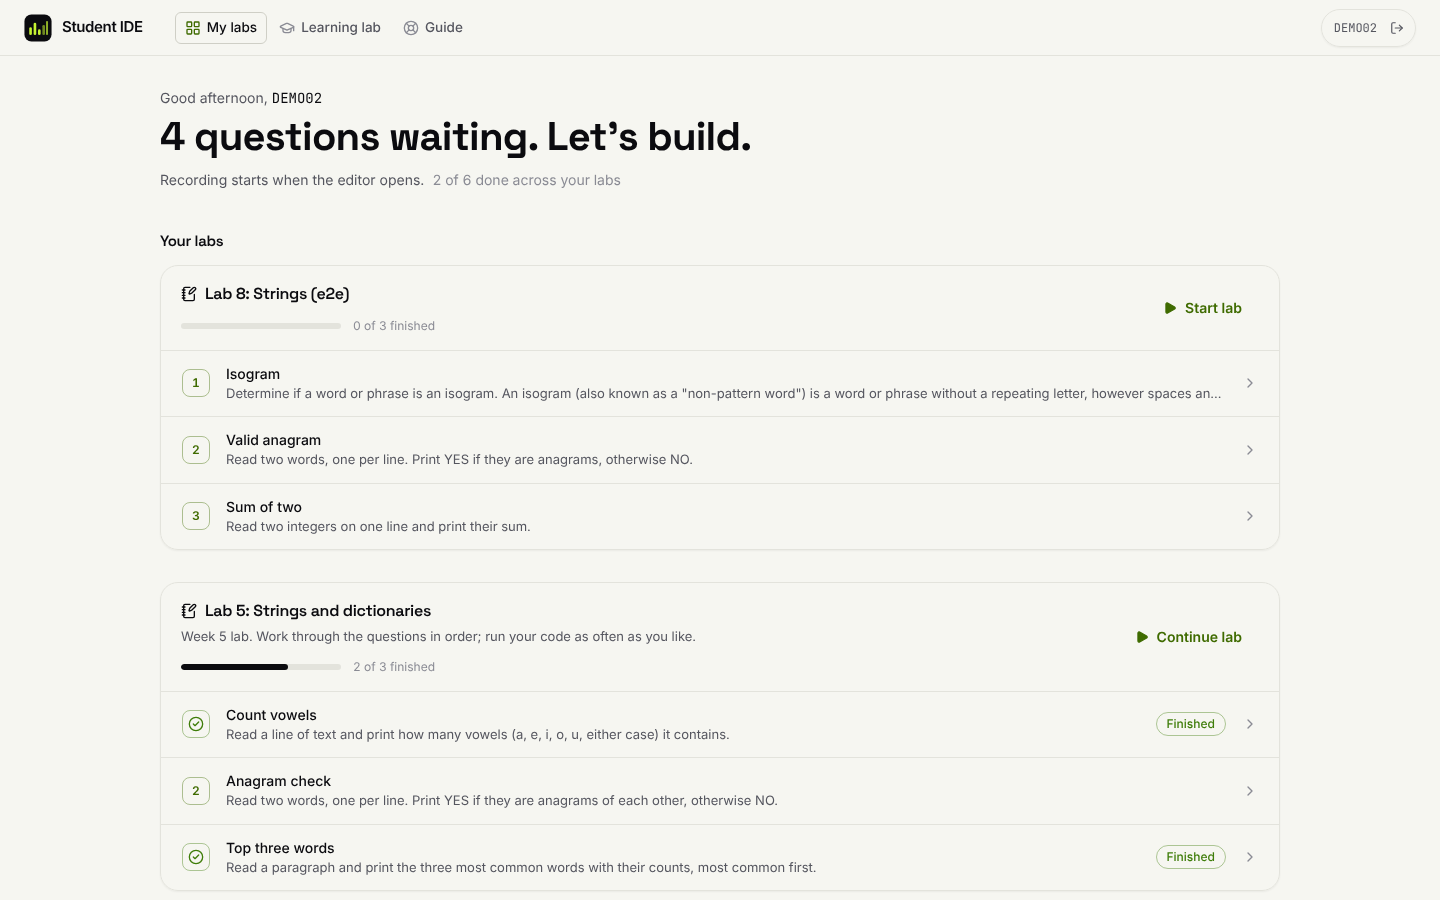
\includegraphics[width=\linewidth]{redesign/acid-night/light-03-student-home}
    \caption{Student home.}
  \end{subfigure}\hfill
  \begin{subfigure}{0.49\textwidth}
    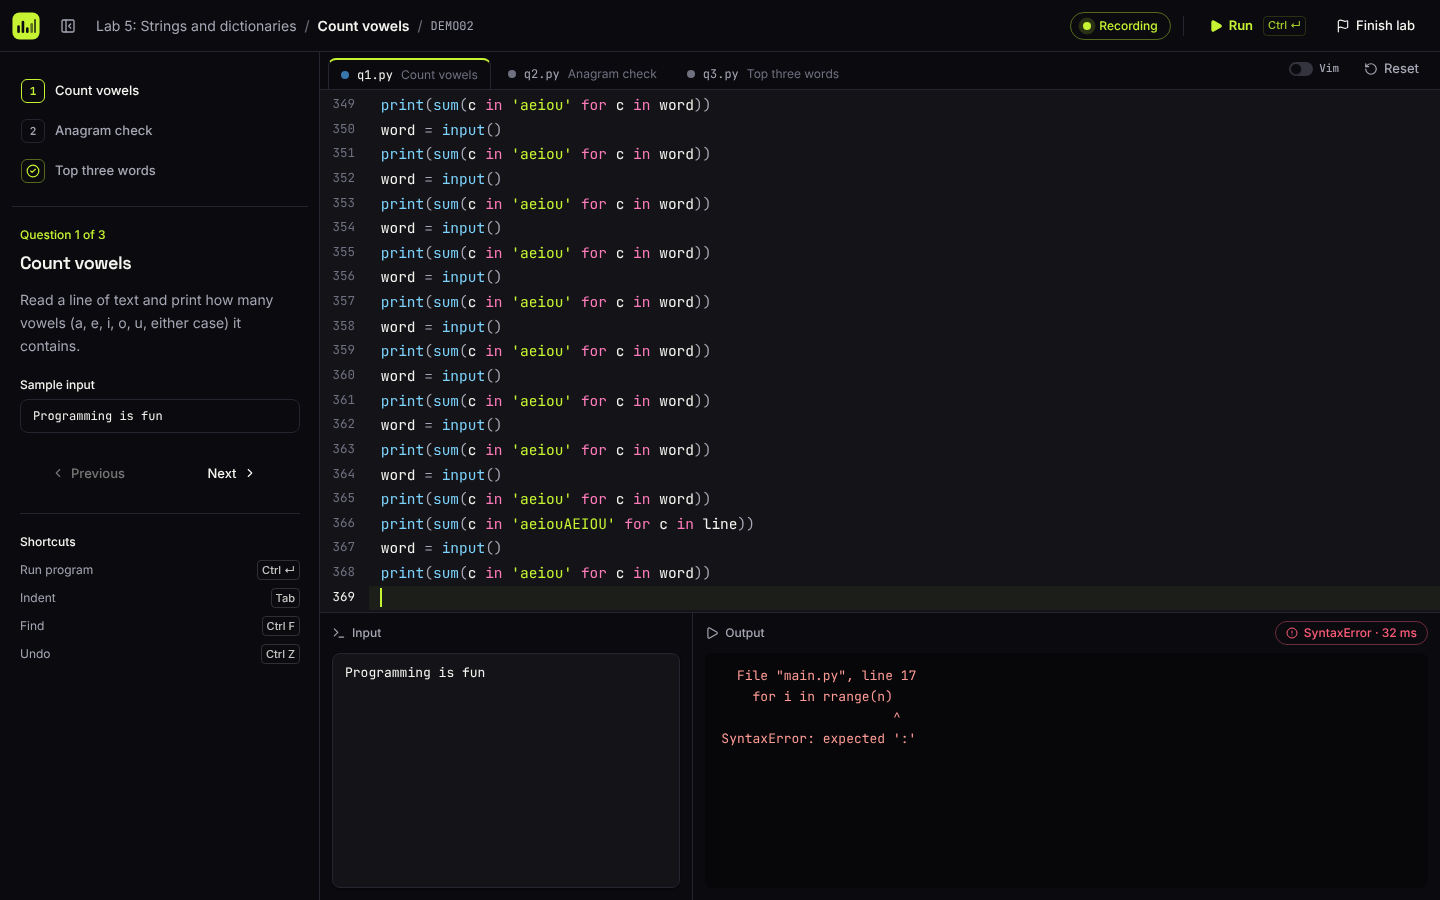
\includegraphics[width=\linewidth]{redesign/acid-night/dark-10-student-workspace}
    \caption{Lab workspace, dark theme.}
  \end{subfigure}
  \caption{The student side after the second redesign.}
  \label{fig:app-ui}
\end{figure}
